\chapter{Spark-SIFT系统的三种性能优化方案}
在上一章节中,本文介绍了整个大规模特征提取系统Spark-SIFT的设计和实现,本章节主要针对Spark-SIFT进行性能优化。第一,是针对Spark-SIFT系统加载大量小图片时,频繁的磁盘IO,读写开销较大问题作出的优化,这该问题的优化上,本文设计了一种新的数据结构来描述图片,将图片转成单条记录的形式,然后将众多的记录合并并且序列化保存供后续操作使用,以提高读写效率;第二,由于Spark的任务划分及分配机制,导致Spark-SIFT系统在处理图片大小差异很大的数据集,会出现负载不均衡的现象,本文提出了分割式特征提取算法以解决处理过程中出现的负载不均衡问题;第三,因为分割式特征提取算法会引用shuffle操作,当处理的图片量很大时,会严重影响系统的性能,因此本文在分割式特征提取算法的基础上改进,提出了shuffle-efficient的特征提取算法,以解决shuffle操作带来的性能问题。

\section{key-value的图片描述数据结构}
因为图片和图片间是分立的,整个数据集是一个个分立的文件组成,spark在加载的时候也只能是一个个加载,如果每个文件很小,文件的数量有多,这情况下读写的效率是很低的。那么怎样才能提高加载时候的性能呢?在spark下处理文本信息会比较多,在处理文本信息时,spark是把一整个文本文件加载进来,然后每一行就是一个基本的并行单元,所以能不能把一张图片看成文本文件中的一行记录,然后很多行记录组成一个大文本,就相当很多个图片合并在一个大文件中,那么一次性就可以加载很多图片了。

针对spark在处理文本文件的启发,我们采用了key-value的方式来描述一张图片,key就是图片的文件名,value就是图片内容的字节流,通过这种方式,就可以用一条记录的形式描述了一张图片,然后将这些记录序列化保存到指定的hdfs目录下,在序列化方式上,Spark-SIFT选用了Hadoop的原生序列化方式,而没有采用Java序列化。这是因为java序列化后产生的内容容量太大,分布式环境中传输时会十分占用带宽,而hadoop序列化产生的内容十分简洁,容量更小,这有助于减少分布式处理时的数据传输量。通过这种将图片转换成记录的形式,spark 在读取该目录时,就可以一次性将目录下的记录加载进来,从能提供了读写的效率。图\ref{fig:kv_image} 显示了整个设计的框架。
\begin{figure}[htp]
\centering
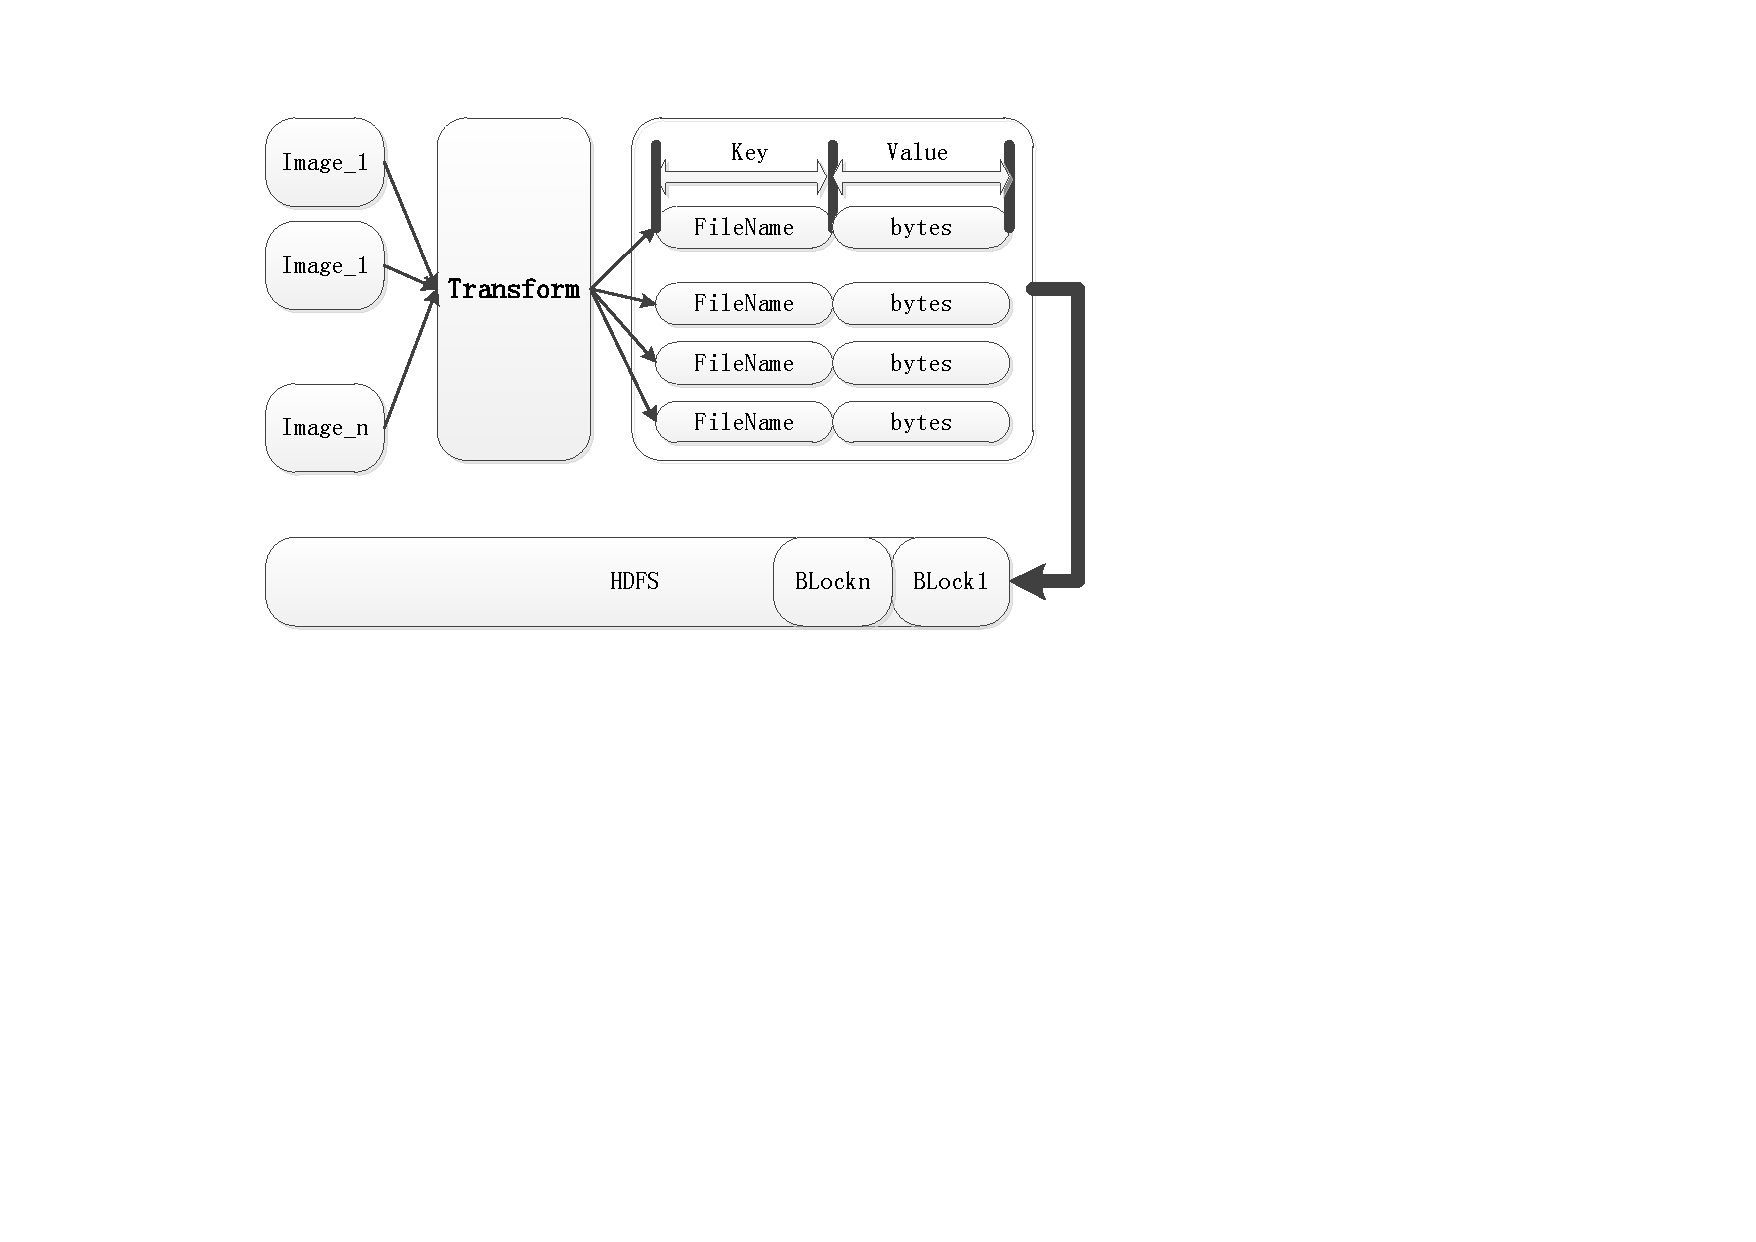
\includegraphics{kv_image}
\caption{key-value描述图片方式}
\label{fig:kv_image}
\end{figure}

具体的实验数据将会在第五章中给出,在此先不进行数据的分析。
\section{分割式图片特征提取算法}
Spark-SIFT有时会出现严重的负载不均衡现象。以提取200 MB图片集合的特征为例,集合中图片的大小为2 MB或4 MB,但其处理时间有时会比处理一个1 GB的图片集合(图片大小在100~200KB之间)还要长。观察Spark的Executors监控页面我们发现,200 MB图片集处理时间较长往往是因为某个Executor的执行速度特别慢,而此时其他Executors都已经完成了分配的任务,处于空闲状态。

导致这个问题的出现有两个原因。首先与SIFT算法自身的特点有关,sift算法的时间复杂度和图片大小相关,为O(N5),并且sift算法的空间复杂度也十分大,并且spark本身也是很耗内存,这样就导致 运行过程中很耗内存,当内存占用过高时,cpu的利用率无法上去,这样就导致运算速度十分慢;其次是spark任务分配机制,spark任务分配按照大小区分,划分时仅考虑了各个任务所处理的图片总容量,而忽略了任务中图片大小的因素。那么,如果图片的大小不一样,一个任务都是大图片,而另外一个是小图片,那么大图片的运行时间会更长,但是spark 分配机制认为只要两个任务是size一样,那么两个任务运行时间基本一样。同时spark分配到executor上的任务,在没有失败的情况下,是不会回收的,尽管有其他空闲的executor,这样就会出现其他executors都是空闲的,只有一个executor 在运算的情况。

针对上面的问题,我们采用分割图片的方式,使图片集中各图片的大小尽可能相同,以适应Spark的任务分配和负载均衡策略,使各个任务的运行时间基本相同。图片分割的具体工作原理如图\ref{fig:segmentation}所示
\begin{figure}[htp]
\centering
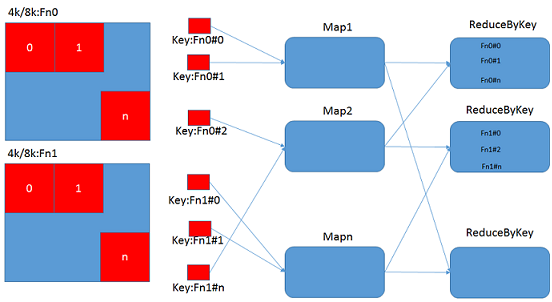
\includegraphics{segmentation}
\caption{分割式特征提取算法}
\label{fig:segmentation}
\end{figure}

本文将分割后得到的图片大小称为分割大小,它会影响特征提取的速度和结果的精度。理论上,分割后的图片越小,每张图片的处理速度越快,但是由于子图之间会产生边缘噪声,导致提取出的特征点存在较大的误差。通过实验,我们选择500×500作为基本分割大小,它既可以保证特征提取的速度足够快,又可以使得结果误差比较小,第五章将详细介绍测试结果和选择依据。

算法流程如图\ref{fig:alg_segmentation}所示,在map任务1,我们将一张图片按照设置的模板大小进行划分,划分为多个子块,每个子块以图片文件名加模块下标,模块的长,模块的宽以及模块的像素内容字节数组四个元素组成。因为在map任务1结束后,一张图片的子块只是位于一个独立的数组中,数组和数组间是分立的,这样并行操作只能在单个数组里面进行,这种情况并行化程度是不高的,因此在map任务1结束后,我们又启用了一个flatMap算子,通过flatMap操作,我们将数组扁平化,将每个数组的元素抽取出来,组成一个大的数组,使得并行化操作在所有图片的子块中执行,这样就可以大大提高并行化程度。当图片子块被扁平化之后,我们又重构了子块的表示方式,在map任务1中,子块的表示方式是(fname,row,col,bytes),在map任务2中,以(fname,(row,col,bytes))的方式表示一个子块,这样子块就可以表示为key-value的形式了,这种表示方式也为后面处理完子块后收集同一张图片的子块提供了方便;在map任务3中,进行子块图片的特征提取工作,在这个任务中,我们还进行key的重构工作,因为之前子块的key是带有下标的,但是在特征提取完之后就不需要带有下标了,因此我们将子块图片的下标去掉,那么同一张图片的子块的key就是一样的,最后提取的出来的特征点集以(fnkey,kpslist.tolist)的形式表示,其中fnkey就是子块图片的所属图片的文件名,kpslist就是子块图片提取的特征点集合,kpslist.tolist表示将其转化成list的形式;在map任务3结束后,我们启动了一个reduceByKey的任务,在该任务中,我们按照key进行value合并,通过这个操作,同一张图片的划分为不同子块提取的特征点集就会收集到一个数组中,数组的每一个元素对应子块提取的特征点集;在最后的一个任务map任务4 中,我们将提取的特征点集进行序列化,最后保存到hdfs中。
\begin{figure}[htp]
\centering
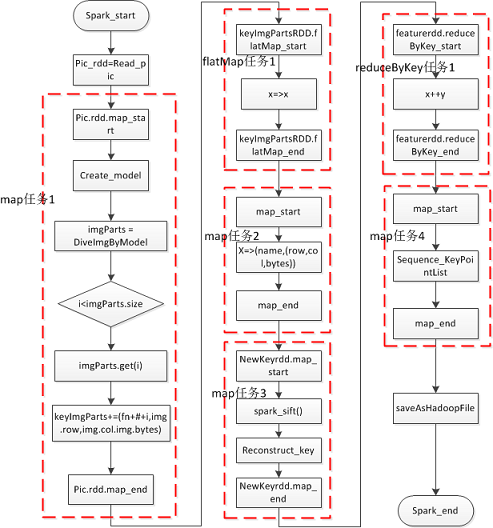
\includegraphics{alg_segmentation}
\caption{分割式特征提取算法流程图}
\label{fig:alg_segmentation}
\end{figure}

子块划分算法如下所示:
\begin{algorithm}[htbp]
  \caption{子块划分算法}
  \label{algDiveModel}
  输入:原始图片,划分模板\\
  输出:子块数组
  \begin{algorithmic}[1]
    \STATE $\mathbf{P}\leftarrow\left(<\alpha>\right)$
    \STATE $\mathbf{S_{a}}\leftarrow\mathbf{P^T}\mathbf{S}\mathbf{P}$
    \FOR{$i=1$ to $S_a$的阶数$m$}
    \STATE $s_i\leftarrow s_i$的第$i$个行向量
    \ENDFOR
    \STATE $\beta_a\leftarrow\lnot \left(s_1\lor s_2\lor \cdots\lor s_m\right)^T$
    \STATE $\beta\leftarrow\mathbf{P}\beta_a$
    \STATE $\gamma\leftarrow\mathbf{A}\beta$
  \end{algorithmic}
\end{algorithm}
\section{shuffle-efficient的特征提取算法}
